% !TEX encoding = ISO-8859-1
\documentclass[bsc]{ufpethesis}

\usepackage{amssymb}
\usepackage{amsmath}
\usepackage{mathtools}
\usepackage{hyperref}
\hypersetup{
    colorlinks,
    citecolor=black,
    filecolor=black,
    linkcolor=black,
    urlcolor=black
}

\usepackage{amsthm}
\newtheorem{definicao}{Defini��o}

%\university{<NOME DA UNIVERSIDADE>}
%\address{<CIDADE DA IES>}
\institute{Centro de Inform�tica}
%\department{Centro de Inform�tica}
\program{Gradua��o em Ci�ncia da Computa��o}
\majorfield{Ci�ncia da Computa��o}
\title{Normaliza��o de ontologias ALC para o uso com o LeanCop}
\date{11 de julho de 2011}
\author{Adriano Silva Tavares de Melo}
\adviser{Frederico Freitas}
%\coadviser{NOME DO(DA) CO-ORIENTADOR(A)}

\begin{document}

%% Parte pr�-textual
\frontmatter
% Folha de rosto
\frontpage
% Portada (apresenta��o)
\presentationpage
% Dedicat�ria
\begin{dedicatory}
Eu dedico esse trabalho a minha m�e, namorada, familiares e amigos.
\end{dedicatory}
% Agradecimentos
\acknowledgements
% !TEX encoding = ISO-8859-1
Gostaria de agradecer � minha m�e, que sempre acreditou em mim, que me deu condi��es de estudar, que abdicou de v�rias coisas ao decorrer de sua vida para dar prioridade aos filhos, que nos incentivou a crescer, que nos ensinou valores, que, em fim, nos amou incondicionalmente.

Agrade�o a todos da minha fam�lia que me apoiaram a estudar e a trilhar caminhos que me deixaram longe, em especial ao meu irm�o, madrinha e av�, que sempre me falam o quanto s�o orgulhosos da minha decis�o de sair da minha cidade para evoluir profissionalmente. Obrigado!

Agrade�o � minha namorada, que tornou essa jornada longe dos amigos e fam�lia mais agrad�vel e feliz.

Agrade�o a Fred, que sempre que precisei se mostrou disposto a ajudar e que me ensinou muito nos �ltimos anos.

Agrade�o a todos que me ajudaram profissionalmente e academicamente, eu n�o teria conseguido chegar at� aqui sem essa ajuda. Obrigado!


\begin{epigraph}[<NOTA>]{<AUTOR>}
<DIGITE AQUI A CITA��O>
\end{epigraph}

\resumo
resumo....
\begin{keywords}
m�todo das conex�es, l�gica de descri��o, l�gica, inteligencia artificial
\end{keywords}

\abstract
\begin{keywords}
<DIGITE AS PALAVRAS-CHAVE AQUI>
\end{keywords}

\tableofcontents
\listoffigures
\listoftables

%% Parte textual
\mainmatter

\chapter{Introdu��o}
\label{ch:introducao}

\section{Contextualiza��o}
A Web � uma das inven��es mais revolucion�rias que o homem j� concebeu. As estimativas de penetra��o mundial, quantidade de informa��es geradas e transa��es financeiras efetuadas sobre essa plataforma s�o n�meros que v�o muito al�m das espectativas de seu criador, Tim Berners-Lee.

Berners-Lee prop�s como seria a Web em mar�o de 1989 ~\cite{BernersLee:1989}, tendo como principais atores documentos interligados atrav�s de hyperlinks. 

 
I have a dream for the Web [in which computers] become capable of analyzing all the data on the Web ? the content, links, and transactions between people and computers. A ?Semantic Web?, which should make this possible, has yet to emerge, but when it does, the day-to-day mechanisms of trade, bureaucracy and our daily lives will be handled by machines talking to machines. The ?intelligent agents? people have touted for ages will finally materialize.

\section{Organiza��o da Disserta��o}

Esta disserta��o est� dividida em seis cap�tulos. No Cap�tulo 1, � apresentada uma 
vis�o geral sobre redes neurais modulares, seus principais benef�cios e motiva��es.
Tamb�m s�o apresentados os principais objetivos desse trabalho. No Cap�tulo 2, s�o
apresentadas as etapas da constru��o de uma rede modular, bem como os principais 
m�todos da literatura utilizados em cada etapa. No Cap�tulo 3 s�o apresentadas as
propostas para decomposi��o de tarefas. No Cap�tulo 4 s�o apresentadas duas propostas 
de arquiteturas modulares, sendo uma delas obtida a partir de uma das propostas para
decomposi��o de tarefas. No Cap�tulo 5 s�o descritos os experimentos, mostrando as
bases de dados utilizadas, os resultados obtidos e as an�lises. Por fim, o Cap�tulo
6 apresenta as considera��es finais sobre o trabalho, bem como propostas de trabalhos
futuros.
%% !TEX encoding = ISO-8859-1
\chapter{Web Ontology Language: OWL}
\label{ch:webontologylanguageowl}

In order to describe the connection method as a formal inference system (in section 4), and the positive matricial normal form used in it, we will briefly describe the notation we use for first order logic, before examining the method. We are presuming readers to be acquainted to first order logic.

\section{Definition 1 (First-order logic syntax).}
The alphabets given by table 1 compose the FOL syntax notation.	? Table 1. First order logic syntax notation.
% !TEX encoding = ISO-8859-1
\chapter{First-Order Logic Preliminaries}
\label{ch:firstorderlogicpreliminaries}

In order to describe the connection method as a formal inference system (in section 4), and the positive matricial normal form used in it, we will briefly describe the notation we use for first order logic, before examining the method. We are presuming readers to be acquainted to first order logic.

\section{Definition 1 (First-order logic syntax).}
The alphabets given by table 1 compose the FOL syntax notation.	? Table 1. First order logic syntax notation.
% !TEX encoding = ISO-8859-1
\chapter{Normaliza��o para o m�todo das conex�es}
\label{ch:normalizacaoparaometododeconexoes}

O m�todo das conex�es proposto por W. Bibel \cite{bibel:1982} � um m�todo para prova autom�tica de teoremas descritos em l�gica de primeira ordem \cite{bibel:1993}. Um dos trabalhos recentes de Freitas et al \cite{Freitas:2010} foi a exten��o desse m�todo para l�gica de descri��o $ALC$.

O artigo intitulado \textit{A Connection Method for Reasoning with the Description Logic ALC} \cite{Freitas:2010} prop�e algoritmos tanto para o m�todo, quanto para a normaliza��o que precisa ser feita na base de conhecimento para que seja poss�vel a representa��o necess�ria para o m�todo das conex�es usando apenas uma matriz. 

O objetivo deste trabalho � implementar algum algoritmo de normaliza��o para o m�todo das conex�es como os citados no texto de Freitas et al. Dois algoritmos foram propostos com esse objetivo \cite{Freitas:2010}; o primeiro utiliza-se de uma tabela com nove regras que devem ser aplicadas � base de conhecimento a fim de obter a forma normal positiva. O segundo, intitulado "\textit{A more complex and efficient normalization}" n�o cria novos s�mbolos durante a sua execu��o, fazendo-o mais eficiente que o primeiro em rela��o ao uso de mem�ria.

No cronograma deste trabalho estava prevista a implementa��o desse segundo algoritmo, por�m, ao decorrer do desenvolvimento, o orientando prop�s um terceiro algoritmo que � ainda mais eficiente em rela��o ao uso de mem�ria, ele � linear em rela��o � quantidade de impurezas na base, enquanto que o "\textit{A more complex and efficient normalization}" � quadr�tico. O restante desse cap�tulo se dedicar� a dar defini��es para o entendimento dos �ltimos dois algoritmos comentados acima e tamb�m descrev� as suas implementa��es.

\section{Tradu��o de ontologias $ALC$ para forma normal disjuntiva}

Para que o leitor consiga entender melhor os algoritmos de tradu��o, alguns conceitos precisam ser fixados. 

M�todos diretos com o m�todo das conex�es s�o formulados para provar que uma f�rmula ou um conjunto de f�rmulas � um teorema, sse cada interpreta��o gerada � uma tautologia. Tautologias normalmente tomam a forma $L \lor \neg L$, nesse caso, a f�rmula precisa estar na Forma Normal Disjuntiva (DNF).

\begin{definicao}[Forma Normal Disjuntiva, cl�usula]
 Uma f�rmula em DNF � uma conjun��o de disjun��es. Ou seja, tomam a forma:

\begin{center}
$\bigcup \limits_{i=1}^{n} C_i$ , ou, $C_1 \lor ... \lor C_n$.
\end{center}

onde cada $C_i$ � uma \textit{cl�usula}. Uma cl�usula � uma conjun��o de literais. Ou seja, tomam a forma:

\begin{center}
$\bigcap \limits_{j=1}^m L_{i, j}$ , ou, $L_{i, 1} \land ... \land L_{i, m}$ , tamb�m representado por $\{ L_{i, 1}, ..., L_{i, m} \}$
\end{center}

onde cada $L_{i, j}$ � um literal, resultando na f�rmula:

\begin{center}
$\bigcap \limits_{i=1}^n \bigcup \limits_{j=1}^m L_{i, j}$ , ou, $(L_{1,1} \land ... \land L_{1,m}) \lor (L_{n, 1} \land ... \land L_{n, m})$
\end{center}

podendo ser chamada tamb�m de forma causal disjuntiva, representada por: 

\begin{center}
$\{\{ (L_{1, 1}, ..., L_{1, m}\}, ..., \{L_{n, 1}, ..., L_{n, m} \}\}$
\end{center}

\end{definicao}

A defini��o acima � a defini��o herdada da l�gica de primeira ordem, para ser v�lida tamb�m para a l�gica de descri��o o conceito de conjun��es e disjun��es deve ser estendido.

\begin{definicao}[Conjun��o ALC]
Uma conjun��o ALC � um literal $L$, uma conjun��o $(E_0 \land , ..., \land E_n)$, ou uma restri��o existencial $\exists x.E$, onde $E$ � uma express�o qualquer em l�gica de descri��o.
\end{definicao}

\begin{definicao}[Disjun��o ALC]
Uma disjun��o ALC � um literal $L$, uma disjun��o $(E_0 \lor , ..., \lor E_n)$, ou uma restri��o de valor $\forall x.E$, onde $E$ � uma express�o qualquer em l�gica de descri��o.
\end{definicao}

\begin{definicao}[Conjun��o ALC pura, Conjun��o ALC n�o pura]
Uma conjun��o ALC pura � uma conjun��o ALC que na forma normal negada n�o cont�m restri��es de valor ($\forall x.E$) e tamb�m n�o cont�m disjun��es $(E \lor , ..., \lor E)$. O conjunto de conjun��es ALC puras � representado por $\hat{C}$. Uma conjun��o ALC n�o pura � uma conjun��o ALC que n�o � pura.
\end{definicao}

\begin{definicao}[Disjun��o ALC pura, Disjun��o ALC n�o pura]
Uma disjun��o ALC pura � uma disjun��o ALC que na forma normal negada n�o cont�m restri��es existenciais ($\exists x.E$) e tamb�m n�o cont�m conjun��es $(E \land , ..., \land E)$. O conjunto de disjun��es ALC puras � representado por $\check{D}$. Uma disjun��o ALC n�o pura � uma disjun��o ALC que n�o � pura.
\end{definicao}

\begin{definicao}[Impureza em uma express�o n�o pura]
Impureza em express�es ALC n�o puras s�o conjun��es em disjun��es n�o puras ou disjun��es em conjun��es n�o puras. O conjunto de impurezas � chamado de \text{conjunto de impurezas ALC} e � representado por $I$.
\end{definicao}

\begin{definicao}[Forma Normal Positiva]
Um axioma ALC est� na Forma Normal Positiva sse ele est� em uma das seguintes formas: 

\begin{center}
i) $A \sqsubseteq \hat{C}$ \\
ii) $\check{D} \sqsubseteq A$ \\
iii) $\hat{C} \sqsubseteq \check{D}$ \\ 
\end{center}

onde A � um conceito at�mico,  $\hat{C}$ � uma conjun��o ALC pura, $\check{D}$ � uma disjun��o ALC pura.

\end{definicao}

O m�todo das conex�es utiliza matrizes para realizar provas de teoremas. No in�cio deste trabalho, ainda n�o era poss�vel de fazer as provas com matrizes aninhadas, ou seja, havia sempre a necessidade de normalizar a base de conhecimento na forma normal positiva (defini��o 7). No entanto, Jens Otten em um trabalho entitulado \textit{A Non-clausal Connection Calculus} \cite{Otten:2011} mostrou como aplicar o m�todo das conex�es sem o passo da normaliza��o. Apesar da recente evoluc�o do m�todo, para o objetivo deste trabalho, ainda � necess�rio fazer a normaliza��o, j� que para l�gica de descri��o, o m�todo ainda n�o foi modificado para usar matrizes aninhadas.

A pr�xima se��o desta monografia descreve o algoritmo proposto pelo orientando para a normaliza��o para a forma normal positiva.


\subsection{Algoritmo Proposto}

Esta se��o da monografia descreve a implementa��o realizada neste trabalho.

O m�todo das conex�es � um m�todo direto, ou seja, uma consulta � base de conhecimento toma verifica se uma f�rmla � uma tautologia e toma a forma $KB \rightarrow \alpha$, onde $\alpha$ � um axioma e $KB$ (\textit{Knowledge base}) � da forma $\bigcap \limits_{i=1}^{n} A_i$, onde $A_i$ tamb�m � um axioma. Expandindo a f�rmula $\neg KB \lor \alpha$, temos:

$\neg \bigcap \limits_{i=1}^{n} A_i \lor \alpha$ [ou, $\neg (A_1 \land ... \land A_n) \lor \alpha$], que pode ser transformada para:

$\bigcup \limits_{i=1}^{n} \neg A_i \lor \alpha$ [ou, $\neg A_1 \lor ... \lor \neg A_n \lor \alpha$]

%, e $\alpha$ ainda � transformada para $\neg \neg\alpha$ para que as regras de normaliza��o tamb�m se apliquem a ela, ficando:

%$\bigcup \limits_{i=1}^{n} \neg A_i \lor \neg \neg \alpha$ [ou, em uma forma por extenso, $\neg A_1 \lor ... \lor \neg A_n \lor \neg \neg \alpha$]

Cada $A_i$ ou $\alpha$ precisam estar na forma normal positiva, ou seja, precisam estar em uma das formas: i) $A \sqsubseteq \hat{C}$, ii) $\check{D} \sqsubseteq A$, ou, iii) $\hat{C} \sqsubseteq \check{D}$, onde $A$ � um conceito, $\hat{C}$ � uma conjun��o pura e $\check{D}$ � uma disjun��o pura.

O primeiro passo do algoritmo � a separa��o de axiomas de equival�ncia de express�es e inclus�es. Os axiomas de equival�ncia ser�o substitu�dos por dois axiomas de inclus�o, e.g., $(A \equiv B \rightarrow A \sqsubseteq B \land B \sqsubseteq A)$.

\begin{algorithm}
\caption{Normalize-Ontology(O)}
\label{alg:normalizeontology}
\begin{algorithmic}[1]
\REQUIRE O: ontologia em l�gica de descri��es $ALC$
\FORALL [A, B s�o express�es, $S_I$ � o conjunto dos axiomas de inclus�o pertencentes a O]{$A \sqsubseteq B \in S_I$}
\STATE Normalize-Axiom ($A \sqsubseteq B$)
\ENDFOR
\FORALL [A, B s�o express�es, $S_{EQ}$ � o conjunto dos axiomas de equival�ncia pertencentes a O]{$A \equiv B \in S_{EQ}$}
\STATE Normalize-Axiom ($A \sqsubseteq B$)
\STATE Normalize-Axiom ($B \sqsubseteq A$)
\ENDFOR
\end{algorithmic}
\end{algorithm}

\textbf{Algorithm \ref{normalizeaxiom}}: O m�todo \textit{Normalize-Axiom($A \sqsubseteq B$)} remove o axioma da ontologia (linha 1), remove as impurezas do dado esquedo (linha 2) e do lado direto (linha 3) do axioma. Caso ele j� esteja na forma normal positiva (linha 3) apenas pela remo��o das impusrezas, ele ser� adicionado � base novamente (linha 5), caso contr�rio, dois axiomas ser�o criados, um com a express�o do lado esquerdo (linha 7) e outro com a express�o do lado direito (linha 8). Caso esses novos axiomas sejam criados, eles j� estar�o na forma normal positiva, j� que uma express�o pura em uma rela��o de inclus�o com um conceito est� na forma normal positiva em qualquer combina��o.

\begin{algorithm}
\caption{Normalize-Axiom ($A \sqsubseteq B$)}
\label{normalizeaxiom}
\begin{algorithmic}[1]
\REQUIRE {$A \sqsubseteq B$: inclus�o de A em B}
\STATE $O = \{O - (A \sqsubseteq B) \} $
\STATE $pure\_left = $ purify $(A, left)$
\STATE $pure\_right = $ purify $(B, right)$
\IF [$S_{PNF}$ � o conjunto das f�rmulas na forma normal positiva]{$(pure\_left \sqsubseteq pure\_right) \in S_{PNF}$}
\STATE $O = \{O \cup (pure\_left \sqsubseteq pure\_right)\} $
\ELSE
\STATE $O = \{O \cup (pure\_left \sqsubseteq N)\} $
\STATE $O = \{O \cup (N \sqsubseteq pure\_right)\} $
\ENDIF
\end{algorithmic}
\end{algorithm}

\textbf{Algorithm \ref{purify}}: O m�todo \textit{purify ($e$, side)} recebe uma express�o em DL $ALC$ e a retorna sem impurezas. O par�metro \textit{side} � necess�rio para remo��o de uma impureza, caso a impureza esteja no lado esquerdo, e.g., $C \sqcap Impurity \sqcap C \sqcap C \sqsubseteq A$, um axioma ser� criado com a impureza do lado esquerdo, e.g., $(C \sqcap NewConcept \sqcap C \sqcap C \sqsubseteq A) \land (Impurity \sqsubseteq NewConcept)$, caso a impureza esteja no lado direito, o comportamento ser� o mesmo mas de forma sim�trica, o seja, um axima do tipo $NewConcept \sqsubseteq Impurity$ ser� criado e a impureza ser� substitu�da por um novo conceito ($NewConcept$).

As impurezas s�o identificadas atrav�s dos m�todos \textit{visit}. A primeira chamada para esse conjunto de m�todos � na linha 3 do m�todo \textit{purity}, caso a express�o de entrada seja uma conjun��o n�o pura, ou na linha 5 do m�todo \textit{purify} caso a express�o seja uma disjun��o n�o pura. O m�todo \textit{visit} em sua implementa��o em Java \footnote{c�digo dispon�vel em: http://github.com/adrianomelo/tg} utiliza o padr�o de projetos visitor, que permite criar novas opera��es sem mudar a defini��o das estruturas de dados \cite{Gamma:1995}.

Uma pilha chamada \textit{expressions\_stack} � usada no m�todo pois em uma implementa��o em Java os m�todos que visitam cada n� da ontologia n�o podem retornar objetos por uma limita��o da biblioteca OWLAPI 3.0 \footnote{documenta��o do m�todo visit: 
http://owlapi.sourceforge.net/javadoc/org/semanticweb/owlapi/model/ OWLClassExpressionVisitor.html} \footnote{javadoc da documenta��o da OWLAPI 3.0: http://owlapi.sourceforge.net/javadoc/}.

\begin{algorithm}
\caption{purify ($e$, side)}
\label{purify}
\begin{algorithmic}[1]
\REQUIRE {e: uma express�o em DL $ALC$}
\REQUIRE {side: � $left$ ou $right$}
\STATE expressions\_stack = STACK()
\IF[$S_{npc}$ � o conjunto das conjun��es n�o puras]{$e \in S_{npc}$}
\STATE visit (expressions\_stack, $e$, side, $conjunction$)
\ELSIF[$S_{npd}$ � o conjunto das disjun��es n�o puras]{$e \in S_{npd}$}
\STATE visit (expressions\_stack, $e$, side, $disjunction$)
\ENDIF
\RETURN POP (expressions\_stack)
\end{algorithmic}
\end{algorithm}

\textbf{Algorithm \ref{alg:extractimpurity}}: O m�todo \textit{Extract-Impurity()} � usado para criar um novo axioma na ontologia com a impureza achada por um dos m�todos \textit{visit}. O par�metro \textit{side} � utilizado para saber em qual lado do axioma a impureza dever� ficar. Ap�s o a cria��o do axioma, o m�todo \textit{Normalize-Axiom()} � chamado com o novo axioma para garantir que ele tamb�m esteja na forma normal positiva.

\begin{algorithm}
\caption{Extract-Impurity ($e$, side)}
\label{alg:extractimpurity}
\begin{algorithmic}[1]
\REQUIRE {e: uma express�o em DL $ALC$}
\REQUIRE {side: � $left$ ou $right$}
\STATE N = NEW-CONCEPT()
\IF{side = $left$}
\STATE $O = \{ O \cup (e \sqsubseteq N)\}$
\STATE Normalize-Axiom($e \sqsubseteq N$)
\ELSE
\STATE $O = \{ O \cup (N \sqsubseteq e)\}$
\STATE Normalize-Axiom($N \sqsubseteq e$)
\ENDIF
\RETURN N
\end{algorithmic}
\end{algorithm}

\textbf{Algorithm 5, 6, 7, 8, 9, 10}: O conjunto de m�todos chamados de \textit{visit} diferem em qual express�o em l�gica de descri��es cada um suporta. O m�todo \textit{visit (stack, $\bigcup \limits^n e_i$, side, kind)}, por exemplo, d� suporte �s uni�es entre express�es.

Quatro par�metros s�o passadados para os m�todos, uma pilha \textit{stack} que � usada para auxiliar a constru��o de uma nova express�o normalizada (os m�todos n�o podem retornar objetos por uma limita��o da OWLAPI 3.0, biblioteca usada na implementa��o em Java). Uma express�o em l�gica de descri��es, que pode ser uma uni�o $\bigcup \limits^n e_i$, interse��o $\bigcap \limits^n e_i$, restri��o  de valor $\forall r E$, restri��o existencial $\exists r E$, complemento $\neg e$ ou conceito $C$. O lado \textit{side} em que a express�o original estava (\textit{left} ou \textit{right}). E o tipo \textit{kind} de express�o que o m�todo estava esperando.

Quando uma conjun��o � passada para o m�todo \textit{visit} e o tipo (\textit{kind}) � igual a \textit{disjunction}, significa que uma impureza foi encontrada e ela deve ser removida pelo m�todo \textit{Extract-Impurity()}. De forma an�loga, quando uma disjun��o � visitada por um dos m�todos \textit{visit} e o tipo esperado � \textit{conjunction}, significa que uma impureza foi encontrada e ela deve ser removida pelo m�todo \textit{Extract-Impurity()}.

\begin{algorithm}
\caption{visit (stack, $\bigcup \limits^n e_i$, side, kind)}
\label{visitunion}
\begin{algorithmic}[1]
\REQUIRE {stack: uma pilha}
\REQUIRE {side: � $left$ ou $right$}
\REQUIRE {$\bigcup \limits^n e_i$: uni�o de express�es $e_i$}
\IF{kind = $conjunction$}
\STATE N = Extract-Impurity($\bigcup \limits^n e_i$, side)
\STATE PUSH (stack, N)
\ELSE
\FORALL {$e_i \in \bigcup \limits^n e_i$}
\STATE visit  (stack, $e_i$, side, kind)
\ENDFOR
\STATE PUSH (stack, $\bigcup \limits^n$ POP(stack))
\ENDIF
\end{algorithmic}
\end{algorithm}

\begin{algorithm}
\caption{visit (stack, $\bigcap \limits^n e_i$, side, kind)}
\label{visitintersection}
\begin{algorithmic}[1]
\REQUIRE {stack: uma pilha}
\REQUIRE {side: � $left$ ou $right$}
\REQUIRE {$\bigcap \limits^n e_i$: interse��o de express�es $e_i$}
\IF{kind = $disjunction$}
\STATE N = Extract-Impurity($\bigcup \limits^n e_i$, side)
\STATE PUSH (stack, N)
\ELSE
\FORALL {$e_i \in \bigcap \limits^n e_i$}
\STATE visit  (stack, $e_i$, side, kind)
\ENDFOR
\STATE PUSH (stack, $\bigcap \limits^n$ POP(stack))
\ENDIF
\end{algorithmic}
\end{algorithm}

\begin{algorithm}
\caption{visit (stack, $\forall r E$, side, kind)}
\label{visitforall}
\begin{algorithmic}[1]
\REQUIRE {stack: uma pilha}
\REQUIRE {side: � $left$ ou $right$}
\REQUIRE {$\forall r E$: restri��o de valor com a rela��o $r$ e a express�o $E$ }
\IF{kind = $conjunction$}
\STATE N = Extract-Impurity($\bigcup \limits^n e_i$, side)
\STATE PUSH (stack, N)
\ELSE
\STATE $E'$ = NNF($E$)
\STATE visit (stack, $E'$, side, kind)
\STATE $E''$ = POP(stack)
\STATE PUSH (stack, $\forall r E''$)
\ENDIF
\end{algorithmic}
\end{algorithm}

\begin{algorithm}
\caption{visit (stack, $\exists r E$, side, kind)}
\label{visitexists}
\begin{algorithmic}[1]
\REQUIRE {stack: uma pilha}
\REQUIRE {side: � $left$ ou $right$}
\REQUIRE {$\exists r E$: restri��o existencial com a rela��o $r$ e a express�o $E$ }
\IF{kind = $disjunction$}
\STATE N = Extract-Impurity($\bigcup \limits^n e_i$, side)
\STATE PUSH (stack, N)
\ELSE
\STATE $E'$ = NNF($E$)
\STATE visit (stack, $E'$, side, kind)
\STATE $E''$ = POP(stack)
\STATE PUSH (stack, $\exists r E''$)
\ENDIF
\end{algorithmic}
\end{algorithm}

\begin{algorithm}
\caption{visit (stack, $\neg e$, side, kind)}
\label{visitexists}
\begin{algorithmic}[1]
\REQUIRE {stack: uma pilha}
\REQUIRE {side: � $left$ ou $right$}
\REQUIRE {$\neg e$: nega��o de uma express�o $e$}
\IF {$E \notin S_{concept}$}
\STATE $e'$ = NNF($\neg e$)
\STATE visit (stack, $e'$, side, kind)
\ELSE
\STATE PUSH(stack, $\neg e$)
\ENDIF
\end{algorithmic}
\end{algorithm}

\begin{algorithm}
\caption{visit (stack, C, side, kind)}
\label{visitexists}
\begin{algorithmic}[1]
\REQUIRE {stack: uma pilha}
\REQUIRE {side: � $left$ ou $right$}
\REQUIRE {C: � um conceito}
\STATE PUSH (stack, C)
\end{algorithmic}
\end{algorithm}

Para uma melhor compara��o da matrizes que s�o geradas com o algoritmo proposto, o exemplo que Freitas et al \cite{Freitas:2010} tamb�m ser� o exemplo deste agoritmo. O axioma de equivalencia no Exemplo 1 � a base de conhecimento usada.


\begin{exemplo}
Deseja-se normalizar o axioma:

\begin{center}
$PizzaMargherita \equiv Pizza \sqcap \exists hasTopping.Tomate \sqcap \exists hasTopping.Muzzarella \sqcap \neg \exists hasTopping.\neg (Tomate \sqcup Muzzarella)$
\end{center}

O primeiro passo do algoritmo (m�todo \textit{Normalize-Ontology()}, p�gina \pageref{alg:normalizeontology}) separa o axioma de equival�ncia em dois axiomas de inclus�o. Obtendo-se ent�o:

\begin{center}
$PizzaMargherita \sqsubseteq Pizza \sqcap \exists hasTopping.Tomate \sqcap \exists hasTopping.Muzzarella \sqcap  \neg \exists hasTopping.\neg (Tomate \sqcup Muzzarella)$

$Pizza \sqcap \exists hasTopping.Tomate \sqcap \exists hasTopping.Muzzarella \sqcap 
\neg \exists hasTopping.\neg (Tomate \sqcup Muzzarella) \sqsubseteq PizzaMargherita$
\end{center}

O m�todo \textit{Normalize-Axiom()} ser� chamado ent�o com cada um dos axiomas obtidos. O lado direito no primeiro axioma e o lado esquerdo do segundo s�o conjun��es, ent�o o m�todo \textit{visit} de interse��es ser� chamado com o kind sendo \textit{conjunction} tanto para a primeira express�o quanto para a segunda.  

Quando o m�todo \textit{visit (stack, $\neg e$, side, kind)} for chamado com a express�o $\neg \exists hasTopping. \neg (Tomate \sqcup Muzzarella)$, tanto para o lado esquerdo, quanto para o lado direito ele a transformar� na express�o $\forall hasTopping.(Tomate \sqcap Muzzarella)$, que � uma disjun��o. Os axiomas que ser�o obtidos s�o:

\begin{center}
$PizzaMargherita \sqsubseteq Pizza \sqcap \exists hasTopping. Tomate \sqcap \exists hasTopping.Muzzarella \sqcap  Extracted1$

$Extracted1 \sqsubseteq \forall hasTopping.(Tomate \sqcup Muzzarella)$

$Pizza \sqcap \exists hasTopping.Tomate \sqcap \exists hasTopping.Muzzarella \sqcap 
Extracted2 \sqsubseteq PizzaMargherita$

$\forall hasTopping.(Tomate \sqcup Muzzarella) \sqsubseteq Extracted2$
\end{center}

Em formato matricial, temos (axiomas 1 e 2):

\[
\small{
\begin{bmatrix}
PM & PM & PM & PM & PM & PM & Extracted1\\
\neg Pizza & \neg hasTopping & \neg Tomate & \neg hasTopping & \neg Muzzarella & \neg Extracted1 & \neg hasTopping\\
 & & & & & & \neg Tomate\\
 & & & & & & \neg Muzzarella\\
\end{bmatrix}
}
\]

e (axiomas 3 e 4):

\[
\begin{bmatrix}
Pizza & \neg hasTopping & Tomate & Muzzarella \\
hasTopping & \neg Extracted2 & \neg Extracted2 & \neg Extracted2 \\
Tomate & & & \\
hasTopping & & & \\
Muzzarella & & & \\
Extracted2 & & & \\
\neg PizzaMargherita & & & \\
\end{bmatrix}
\]

O algoritmo de Freitas et al \cite{Freitas:2010} chegou �s mesmas matrizes. O que indica que ambos s�o lineares em rela��o �s impurezas deste exemplo.

\end{exemplo}

\begin{exemplo}
No exemplo dado por Freitas et al \cite{Freitas:2010}, o seu algoritmo se comportava de forma linear (em espa�o) em rela��o �s impurezas nas express�es. Por�m, com o caso $\hat{C} \sqsubseteq \hat{D}$, onde $\hat{C}$ e $\hat{D}$ s�o conjun��es puras, o algoritmo se comporta de forma quadr�tica em rela��o a mem�ria.

O algoritmo proposto ir� dividir o axioma em dois, ficando $\hat{C} \sqsubseteq A$, e $A \sqsubseteq \hat{D}$. J� o algoritmo de Freitas et al, ir� construir v�rios axiomas, um para cada express�o do lado direito, e.g., \{$\hat{C} \sqsubseteq D_1, \hat{C} \sqsubseteq D_2, ..., \hat{C} \sqsubseteq D_{m-1}, \hat{C} \sqsubseteq D_m$\}. O que ir� resultar em uma matriz do tipo:

\[
\begin{bmatrix}
C_1 & C_1 & \hdots & C_1 & C_1 \\
C_2 & C_2 & \hdots & C_2 & C_2 \\
\vdots & \vdots & \ddots & \vdots & \vdots \\
C_{n-1} & C_{n-1} & \hdots & C_{n-1} & C_{n-1} \\
C_n & C_n & \hdots & C_n & C_n  \\
\neg D_1 & \neg D_2 & \hdots & \neg D_{m-1} & \neg D_m
\end{bmatrix}
\]

enquanto que o algoritmo proposto ir� produzir uma matriz do tipo:

\[
\begin{bmatrix}
C_1 & A \\
C_2 & \neg D_1 \\
\vdots & \neg D_2 \\
C_{n-1} & \vdots \\
C_n & \neg D_{m-1} \\
\neg A & \neg D_m \\
\end{bmatrix}
\]

\end{exemplo}

\subsection{Algoritmo Original}

Esta se��o cont�m o algoritmo escrito por Freitas et al \cite{Freitas:2010} para a normaliza��o de bases de conhecimento em l�gica de descri��o $ALC$. A figura 3.1 descreve o m�todo \textit{Normalize-Ontology ()}, que chama os m�todos \textit{Normaize-LHS ()} e \textit{Normalize-RHS ()} caso o lado esquerdo e direito, respectivamente,  n�o estejam normalizados para cada axioma da ontologia.

Os m�todos \textit{Normalize-LHS ()} e \textit{Normalize-RHS} s�o duais, ou seja, possuem a mesma l�gica mas com o sentido invertido. A figura 3.2 mostra o pseudoc�digo do m�todo \textit{Normalize-LHS()} e a figura 3.3 mostra o pseudoc�digo do m�todo \textit{Normalize-RHS}.

\begin{figure}
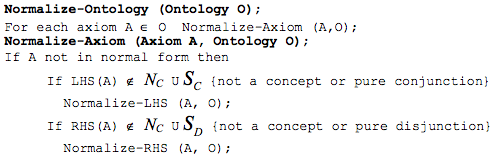
\includegraphics[scale=0.7]{../imagens/normalize.png}
\caption{M�todo \textit{Normalize-Ontology ()}}
\label{fig:normalizeontology}
\end{figure}

 \begin{figure}
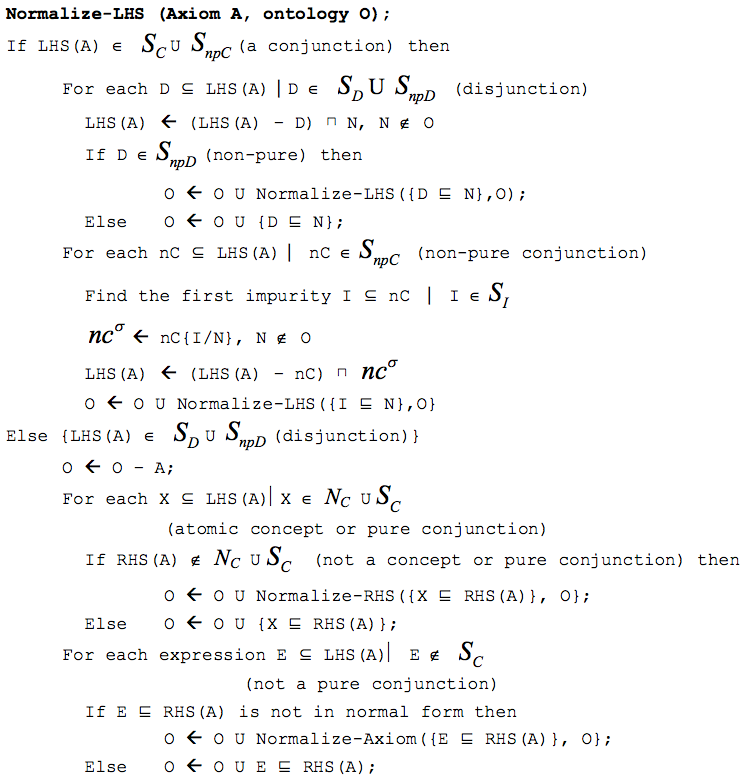
\includegraphics[scale=0.52]{../imagens/normalizelhs.png}
\caption{M�todo \textit{Normalize-LHS ()}}
\label{fig:normalizelhs}
\end{figure}

 \begin{figure}
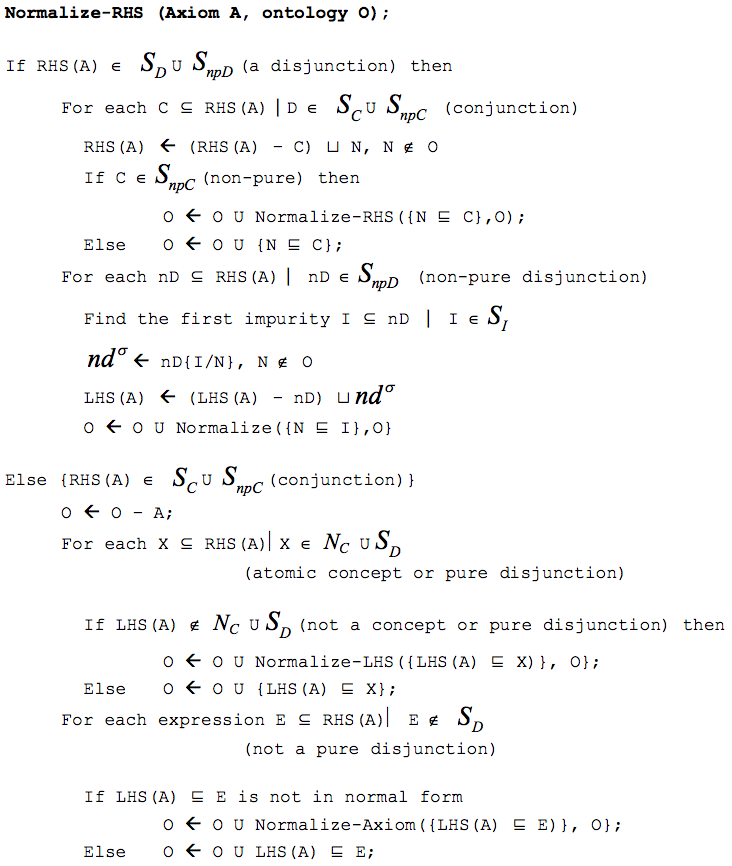
\includegraphics[scale=0.52]{../imagens/normalizerhs.png}
\caption{M�todo \textit{Normalize-RHS ()}}
\label{fig:normalizerhs}
\end{figure}

Note que o primeiro algoritmo da se��o 3.1.1 e a figura 3.1 s�o praticamente o mesmo, por�m, o primeiro diferencia dentro do m�todo os axiomas de equival�ncia e inclus�o. No artigo de Freitas et al \cite{Freitas:2010} � citado que isso deve ser feito, mas n�o explicita no algoritmo.

% !TEX encoding = ISO-8859-1
\chapter{leanCoP}
\label{ch:translation}

O leanCoP � um provador autom�tico de teoremas para l�gica de primeira ordem escrito em Prolog \cite{Otten:2003}. Em testes realizados com a biblioteca TPTP \cite{SS98}, o leanCoP mostrou boa performance, mesmo comparado a provadores de teoremas que s�o estado da arte. Dentre os 2200 problemas inclusos na biblioteca TPTP, o leanCoP foi capaz de resolver 667 (30.3\%), 532 problemas a mais que o leanTAP \cite{leantap:1994} e 932 a menos que o Otter \cite{otter:1995}. 

O objetivo do uso do leanCoP neste trabalho � validar o algoritmo de normaliza��o descrito em 3.1.1, caso o leanCoP consiga ser usado com a base de conhecimento descrita em $ALC$, significa que os axioms da base est�o na forma normal positiva.

� import�nte notar que a ontologia OWL, documento que cont�m os axiomas da base de conhecimento, � descrita em l�gica de descri��o. Algumas ferramentas se mostraram necess�rias para que essa base em OWL fosse usada com o leanCoP. Primeiro, a ontologia � convertida para o formato TPTP a partir da biblioteca owlapi 1.0 \footnote{download: http://sourceforge.net/projects/owlapi/files/OWL\%20API\%20\%28OWL\%201.0\%29/}, o arquivo gerado passa ent�o por uma transforma��o para que use a linguagem de l�gica de primeira ordem do TPTP. Ap�s essa transforma��o, os axiomas da base podem ser utilizadas pelo leanCoP. 

Os c�digos abaixo mostram exemplos da linguagem usada pelo leanCoP:

\begin{verbatim}
fof(axiom_13,axiom,(
    ! [X] : 
      ( iAB(X)
    <=> ( iA(X)
        | iB(X) ) ) )). 
\end{verbatim}

O exemplo acima � um axioma expresso em l�gica de primeira ordem que � equivalente a: 

\begin{center}
$\forall x (AB(x) \iff A(x) \lor B(x))$ 
\end{center}

A owlapi, biblioteca que transforma de OWL para TPTP, define em l�gica de primeira ordem alguns conceitos b�sicos que s�o necess�rios para que os teoremas separem o dom�nio das int�ncias de classes do dom�nio dos tipos pre-definidos em OWL. o exemplo de c�digo abaixo mostra tr�s dos onze axiomas que s�o gerados pela biblioteca com esse objetivo:

\begin{verbatim}
fof(axiom_0,axiom,(
    ! [X] :
      ( abstractDomain(X)
      | dataDomain(X) ) )).

fof(axiom_1,axiom,(
    ? [X] : abstractDomain(X) )).

fof(axiom_2,axiom,(
    ? [X] : dataDomain(X) )).
\end{verbatim}

O primeiro axioma � igual a $\forall x (abstractDomain(x) \lor dataDomain(x))$, ou seja, todos os elementos do dom�nio ou s�o $abstractDomain$ ou $dataDomain$. O segundo axioma � igual a $\exists x (abstractDomain(x))$, ou seja, o dom�nio $abstractDomain$ n�o � vazio. E o terceiro axioma do exemplo � igual a $\exists x (dataDomain(x))$, ou seja, o dom�nio $dataDomain$ tamb�m n�o � vazio. Abaixo est�o todos os axiomas que s�o b�sicos para todas as bases:

\[	\forall x (abstractDomain(x) \lor dataDomain(x))	\]
\[	\exists x (abstractDomain(x))	\]
\[	\exists x (dataDomain(x))	\]
\[	\forall x \neg (abstractDomain(x) \land dataDomain(x))	\]
\[	\forall x (owlThing(x) \implies abstractDomain(x))	\]
\[	\forall x (owlNothing(x) \implies abstractDomain(x))	\]
\[	\forall x (abstractDomain(x) \implies owlThing(x))	\]
\[	\forall x \neg (owlNothing(x))	\]
\[	\forall x (xsd\_string(x) \implies dataDomain(x))	\]
\[	\forall x (xsd\_integer(x) \implies dataDomain(x))	\]
\[	\forall x (dataDomain(x) \implies \neg (xsd\_string(x) \land xsd\_integer(x))	\]

Para fazer alguma atividade de racioc�nio a partir dessa base, um n�mero exponencial de consultas deveria ser gerado. Subsuns�o, por exemplo, consistir� em perguntar se cada conceito pode ser sub-classe de outro conceito.

Devido a essa solu��o ser muito ineficiente, devido � quantidade transforma��es de arquivos que cada consulta deveria gerar, essa atividade de consulta acaba fugindo do escopo desse projeto, que � a implementa��o do algoritmo de normaliza��o para o M�todo das Conex�es com ontologias $\mathcal{ALC}$.


%\section{Definition 1 (First-order logic syntax).}






% !TEX encoding = ISO-8859-1
%\chapter{Conclus�o e trabalhos futuros}
%\label{ch:conclusaoetrabalhosfuturos}

\section{Conclus�o}
Os resultados de boa performance do leanCoP para l�gica de primeira ordem d�o ind�cios que o m�todo das conex�es pode ganhar espa�o entre os m�todos de prova para l�gica de descri��o. Como a w3c \footnote{site: http://w3.org} ainda n�o definiu uma tecnologia padr�o para a camada de l�gica e prova da Web Sem�ntica, trabalhos como o que este est� inserido s�o de import�ncia estrat�gica para a Web, eles desenvolvem solu��es que poder�o ser adotados em larga escala pelo mundo.

O leanCoP foi envolvido neste trabalho para realizar atividades de racioc�nio, como subsun��o e equival�ncia, ap�s a normaliza��o da base de conhecimento. O leanCoP � escrito em Prolog e as APIs de manipula��o de ontologias OWL s�o escritas em Java. Para fazer o leanCoP usar como base de conhecimento as ontologias OWL normalizadas, foi utilizado o formato TPTP como linguagem intermedi�ria. Por�m, para fazer as atividades de racioc�nio de forma autom�tica, um n�mero exponencial de arquivos deveriam ser gerados em TPTP para serem usados com o leanCoP. Al�m disso, um trabalho de \textit{parsing} desses arquivos deveria ser realizado para adicionar cada consulta � base de conhecimento de cada arquivo, o que se mostrou fora do escopo do projeto. O leanCoP foi utilizado ent�o para fazer simples checagem de consist�ncia na base de conhecimento, que traz como efeito colateral a valida��o da corretude do algoritmo de normaliza��o.

Na proposta inicial deste trabalho estava prevista a implementa��o do algoritmo de normaliza��o de Freitas et al \cite{Freitas:2010}, por�m, apesar do algoritmo n�o incluir novos s�mbolos � base de conhecimento, n�o � f�cil de ser entendido. A se��o 3.1.1 mostra em pseudo-c�digo a implementa��o que foi feita neste trabalho. O algoritmo foi produzido devido a uma provoca��o de simplificar o algoritmo de Freitas et al \cite{Freitas:2010}. O objetivo dos algoritmos � o mesmo, traduzir os axiomas de uma ontologia ALC para a forma normal positiva, mas o algoritmo da se��o 3.1.1 al�m de ser mais simples de ser implementado, faz a matriz gerada ap�s a normaliza��o consumir menos mem�ria, o que foi uma grande contribui��o. A redu��o do uso de mem�ria vai impactar no tempo de execu��o do m�todo das conex�es para l�gica de descri��o, j� que a busca pelos caminhos na matriz vai ser reduzido.

\section{Trabalhos futuros}

Este trabalho n�o contempla todos os constructos de OWL, nem sequer de OWL Lite, j� que � limitada � familia ALC. Trabalhos futuros ser�o para estender o algoritmo de normaliza��o para incluir restri��es com cardinalidade, dom�nio e contradom�nio de propriedades, disjun��o entre classes e assim por diante.

Este trabalho � apenas um dos m�dulos necess�rios para a implementa��o de um raciocinador escrito em java que use o m�todo das conex�es. O algoritmo em si que procura pelas conex�es, ou caminhos, ainda n�o foi implementado.

E, por fim, quando o m�todo das conex�es estiver formalizado para uma fam�lia de DL que seja equivalente a uma fam�lia de OWL e a sua implementa��o estiver finalizada, poder� haver um trabalho para integrar o raciocinador a editores de ontologias existentes no mercado, como o Prot�g�.



%% Parte p�s-textual
\backmatter

\appendix
% \include{apendice1}

% Bibliografia
% � aconselh�vel utilizar o BibTeX a partir de um arquivo, digamos "biblio.bib".
% Para ajuda na cria�?o do arquivo .bib e utiliza�?o do BibTeX, recorra ao
% BibTeXpress em www.cin.ufpe.br/~paguso/bibtexpress
\nocite{*}
\bibliographystyle{alpha}
\bibliography{../referencias/referencias}

% Inclui uma pequena nota com refer�ncia � UFPEThesis
% \colophon

%% Fim do documento
\end{document}
